\documentclass[dvipdfmx,12pt]{beamer}
\usepackage{newtxtext,newtxmath}
\usepackage{lipsum}
\usetheme{CambridgeUS}
\usepackage{bxdpx-beamer}
\usepackage{pxjahyper}
\usepackage{minijs}
\usepackage{mathpazo}
\usepackage{amsmath,amssymb}
\usepackage{graphicx}
\usepackage{array}
\usepackage{tikz}
\usepackage{wrapfig}
\usepackage{float}
\usepackage{here}
\usepackage{lscape}
\setbeamertemplate{navigation symbols}{}

\title{Reference Dependence and Monetary Incentive}
\subtitle{-Evidence from Major League Baseball-}
\author{Reio TANJI\footnote{ot.shunie.rt@gmail.com} }
\date{Mar. 5th, 2019}
\institute{Osaka University, Graduate Scool of Economics}

\begin{document}

\begin{frame}\frametitle{}
  \titlepage
\end{frame}

\section*{Table of Contents}
\begin{frame}\frametitle{Contents}
  \tableofcontents
\end{frame}

\section{Introduction}

\begin{frame}\frametitle{Abstract}
  \begin{itemize}
    \item This paper explored the relationship between observed reference dependent behavior and monetary incentives.

    \item Specifically, this paper used performance stats and contract design of Major League Baseball (MLB) players, and identified their salary determination procedure.

    \item MLB players have round-number reference dependence about their performance indexes, which is not caused by their monetary incentives.

  \end{itemize}
\end{frame}

\begin{frame}\frametitle{Research Question}
  \begin{itemize}
    \item How observed reference dependence is related to the monetary incentives?

    \item What factor lead individuals to recognize a reference point and make effort to achieve it?
  \end{itemize}
\end{frame}

\begin{frame}\frametitle{Background}

  \begin{itemize}
    \item Reference dependence is one of the two main characteristcs of the prospect theory:

    Individuals evaluate outcomes by the relative value to their internal benchmarks, or reference point, not by their absolute ones

    \item There are a lot of subsequent researches that shows the evidence for the reference dependence in field and laboratory settings.
  \end{itemize}

\end{frame}

\begin{frame}\frametitle{Literature}
  \begin{itemize}
    \item There are also some researches that use cases from athletes' decision making.
  \end{itemize}

    \begin{block}{Reference Dependence of Athletes}
      \begin{itemize}
        \small
        \item Pope and Schweizer (2011, AER) pointed out that for the professional golf players regard ``par'' as a reference point, which results in the different probability of success in their putts.

        \item Allen et al. (2016) identified existance of reference point dependence of marathon runners, using data about the finish time of enormous number of races in the United States.

        $\Rightarrow$ Runners try to goal before the round numbers, and it results in observed excess mass, or ``bunching'' around 4 hours.

      \end{itemize}
    \end{block}
\end{frame}

\begin{frame}\frametitle{Literature}
  \begin{itemize}
    \item Pope and Simonsohn (2011) picked up the case of Major League Baseball (MLB) players about the observed attitude to their performance indexes.

    \item MLB position players make effort to manipulate their batting-average (AVG), in order to meet their internal goals: .300

    \item As a result, there is observed excess mass, or ``bunching'' around .300 of AVG.
  \end{itemize}
  \begin{figure}
    \small
    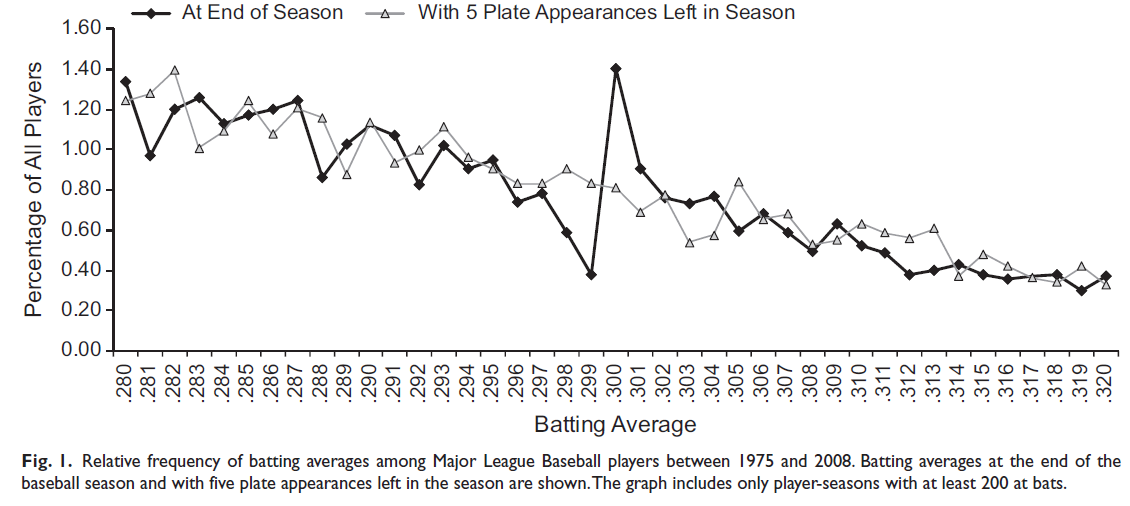
\includegraphics[keepaspectratio, scale = 0.33]{graphs/PS_fig1}
    \caption{Excess Mass Around .300 (quated from Pope and Simonsohn (2011))}
    \label{PS_fig}
  \end{figure}
\end{frame}

\begin{frame}\frametitle{Contribution}
  \begin{itemize}
    \item The case of MLB is different from that of marathon in that players are professinal, and receive salary, or monetary rewards.

    \item There may exist an economically reasonable factor that leads them to bunching:

    The fact that a player achieves round-number of a performance index (such as .300 of batting-average) itself is to be rewarded

    \item The contribution of our research is to explore this: examine if there exists any monetary incentives that make players make effort to the cutoff point.
  \end{itemize}
\end{frame}

\section{Theoretical Framework}

\begin{frame}\frametitle{Benefit of Better Performance}
  This paper assume two ways of specification of players benefit of better number of indexes.
  \begin{enumerate}
    \item Players yield internal benefits that depend on their performance index $X$, $b(X, Z)$. $Z$ is other observed player-specific characteristcs, such as age, position, and so on.

    \item Players receive monetary reward determined by $f(X, Z)$, and they regard this as their benefit for better perfrmance.
  \end{enumerate}

  The second case corresponds to the assumption that monetary incentive leads them to bunching.
\end{frame}

\begin{frame}\frametitle{Effort Cost for Better Performance}
  \begin{itemize}
    \item On the other hand, getting better performance requires them to make some additional effort:

    $X$ is determined by the players' effort level $e$.

    \item Then, effort cost $c(.)$ is defined with $c'() > 0$ and $c"(.) >0$. Note that $c(.)$ differs from player to player.

    $\Rightarrow$ Player $i$ at season $t$'s objective function of the maximization problem is:

    \begin{enumerate}
      \item $U_{it} = b(X(e_{it}), Z_{it}) - c_{it}(e_{it})$

      \item $U_{it} = f(X(e)_{it}, Z_{it}) - c_{it}(e)$
    \end{enumerate}

    This specification way follows that of Allen et al (2016).
  \end{itemize}
\end{frame}

\begin{frame}\frametitle{Assumptions for Excess Mass}
  \begin{itemize}
    \item There are two possible assumptions about functional form of $b(.,.)$ and $f(.,.)$, which leads to bunching around a reference point $r$.

  \end{itemize}

  \begin{block}{Functional Features of Bunching}
    \begin{enumerate}
      \footnotesize
      \item ``Notch'' at $r$.
      \begin{align*}
        \lim_{\epsilon \to 0} b_r (r + \epsilon) & \neq
        \lim_{\epsilon \to 0} b_r (r - \epsilon) \\
        \lim_{\epsilon \to 0} f_r (r + \epsilon) & \neq
        \lim_{\epsilon \to 0} f_r (r - \epsilon)
      \end{align*}

      \item ``Kink'' at $r$.
      \begin{align*}
        \lim_{\epsilon \to 0} b'_r (r + \epsilon) & \neq
        \lim_{\epsilon \to 0} b'_r (r - \epsilon) \\
        \lim_{\epsilon \to 0} f'_r (r + \epsilon) & \neq
        \lim_{\epsilon \to 0} f'_r (r - \epsilon)
      \end{align*}
    \end{enumerate}
  \end{block}
\end{frame}

\begin{frame}
  \begin{tabular}{lrr}
    \begin{minipage}[H]{0.4\textwidth}
      \begin{figure}[H]
        \begin{tikzpicture}[domain = 0:4, samples = 200, >= stealth]
          \draw[->](-0.5, 0) -- (4.2, 0) node[right]{$X$};
          \draw[->](0, -0.5) -- (0, 3.7) node[above]{$f(X),b(x)$};
          \draw[-](2.2, -0.1) -- (2.2, 0.1);
          \draw[domain=0:2.2,samples=200,>=stealth] plot (\x, {sqrt(\x)});
          \draw[domain=2.2:4.1,samples=200,>=stealth] plot (\x, {sqrt(\x) + 0.8});
          \draw (0, 0) node[below left]{O};
          \draw (2.2, -0.3) node {$r$};
      \end{tikzpicture}
      \scriptsize
      \caption{"Notch" at the reference point}
      \label{jump}
    \end{figure}
  \end{minipage} &
  \begin{minipage}[H]{0.5\textwidth}
    \begin{figure}[H]
      \begin{tikzpicture}
        [domain = -2:2, samples = 200, >= stealth]
        \draw[->] (-2,0) -- (2,0) node[right]{$X$};
        \draw[->] (0,-2) -- (0,2) node[above]{$f(X), b(X)$};
        \draw plot[domain = 0:1.7] (\x, \x);
        \draw plot[domain = -0.9:0] (\x, {2 * \x});
        \draw (0,0) node [below right] {$r$};
      \end{tikzpicture}
      \scriptsize
      \caption{"Kink" at the reference point}
      \label{kink}
    \end{figure}
  \end{minipage}
 \end{tabular}
\end{frame}

\begin{frame}
  \begin{itemize}
    \item Suppose there exists bunching around a possible reference point such as .300 of batting-average, $b$ or $f$ should have functional forms mentioned above.

    \item This paper test if $f$ has such features or not:

    If the players' salary jump or kink at the reference point, then it works as the cause that lead them to bunching.
  \end{itemize}
\end{frame}


\section{Methodology and Data}
\begin{frame}\frametitle{Flow of Identification}
  \begin{enumerate}
    \item First, we follow Pope and Simonsohn (2011):

    identify bunching around round-numbers of various indexes.

    -- We test not only batting-average, but also other indexes of position player.

    \item Then, we test if there exists additional monetary bonus where bunching was observed.
  \end{enumerate}
\end{frame}

\begin{frame}\frametitle{Identification of Bunching}
  \begin{tabular}{lr}
    \begin{minipage}[H]{0.45\textwidth}
      \small
      \begin{itemize}
        \item We exploit the McCrary (2007)'s manipulation test, which is used in regression discontinuity design.

        \item Make local approximation of the histgram of the variable of interest, and calculate the predicted values of $f(r)$ at the cutoff point, from both above and below there.
      \end{itemize}
    \end{minipage}
    &
    \begin{minipage}[H]{0.5\textwidth}
      \begin{figure}
        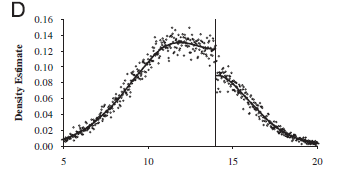
\includegraphics[keepaspectratio, scale = 0.8]{graphs/McCrary_figD.png}
        \caption{Discontinuous frequency (quated from McCrary(2007))}
        \label{McC}
      \end{figure}
    \end{minipage}
  \end{tabular}
\end{frame}

\begin{frame}\frametitle{Identification of Reward Function}
  \begin{itemize}
    \small
    \item Notch of the contract design is tested by local-linear regression:
    \begin{align*}
      \footnotesize
      w_{it} = & \beta_0 + \beta_1 \text{PERF}_{it} + \beta_2 \text{ABOVE}_{it} \\
      \text{where} \\
      w_{it}: & \text{ log salary of the next season} \\
      \text{PERF}_{it}: & \text{ performance index} \\
      \text{ABOVE}_{it}: & \text{ indicator for achievement}
    \end{align*}

    \item Also, kink is examined by introducing the interaction term of $\text{PERF}_{it}$ and $\text{ABOVE}_{it}$
    \[
    \footnotesize
    w_{it} = \beta_0 + \beta_1 \text{PERF}_{it} + \beta_2 \text{ABOVE}_{it} + \beta_3 \text{PERF}_{it} \times \text{ABOVE}_{it}
    \]

    We also conduct analysis including other performance and other player specific charactaristics.
  \end{itemize}
\end{frame}

\begin{frame}\frametitle{Data Description}
  We obtain information about the players' stats (indexes) and annual salary.
  \begin{itemize}
    \item Stats Data
    \begin{itemize}
      \item From \textit{FanGraphs}

      \item Play stats from 1957 to 2018

      \item We restrict the sample to the players with at least 200 plate-appearances $N=18143$ (62 seasons $\times$ players)
    \end{itemize}
    \item Salary Data
    \begin{itemize}
      \item From \textit{USA TODAY} and \textit{Baseball References}

      \item Contract information from 1987 to 2017 $N=8915$(31 seasons $\times$ players)
      \begin{itemize}
        \item Fixed part of the salary of each player

        \item Information about possession of free agency, the right to negotiate any team in MLB.
      \end{itemize}
    \end{itemize}
  \end{itemize}
\end{frame}

\section{Results}

\begin{frame}\frametitle{Results}
  \huge
  To be written...
\end{frame}

\begin{frame}\frametitle{Bunching: McCrary's Test}
  \begin{figure}
    \centering
    \caption{Histgram of Batting-Average}        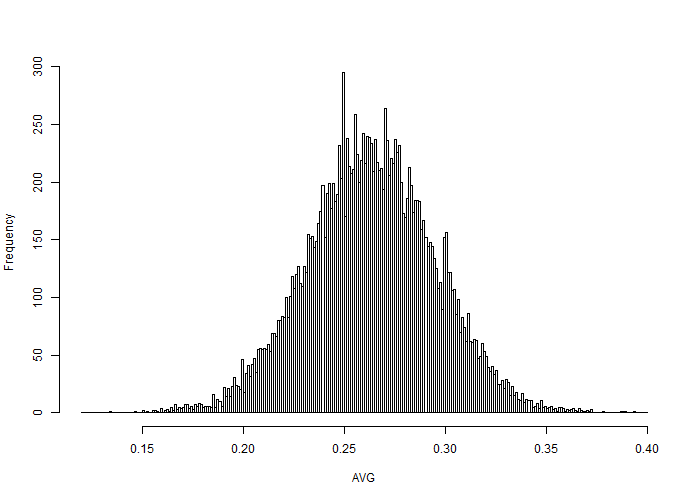
\includegraphics[keepaspectratio, scale = 0.35, angle=0]{graphs/hist_AVG_all.png}
    \label{AVG_Histgram}
  \end{figure}
\end{frame}

\begin{frame}
  \begin{figure}
    \centering
    \caption{Discontinuity at .300 of AVG}
    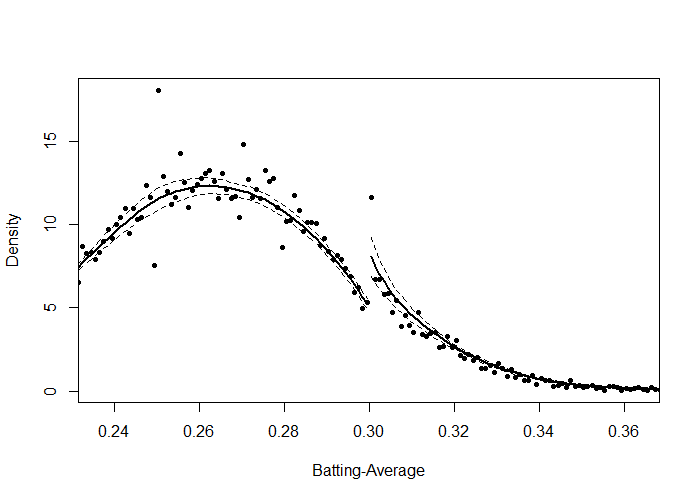
\includegraphics[keepaspectratio, scale = 0.5, angle = 0]{graphs/AVG_300.png}
    \label{DCdensity_AVG_300}
  \end{figure}
\end{frame}

\begin{frame}
  \begin{table}
    \tiny
    \centering
    \caption{Test for Bunching, leastPA $= 200$}
    \begin{tabular}{lcccccc}\hline
      index & type & cutpoint & binsize & bandwidth & $\theta$ & $z$
      \\ \hline \hline
      AVG & rate & .300 & .001 & .019 &  .499 & 7.442*** \\
      & & & & & (.067) & \\
      & & .250 & .001 & .024 & .212 & 5.061*** \\
      & & & & & (.042) & \\
      OBP & rate & .350 & .001 & .024 &  .139 & 2.854** \\
      & & & & & (.049) &  \\
      HR & cumulative & 20 & 1 & 5.309 & .259 & 3.465*** \\
      & & & & & (.075)  & \\
      RBI & cumulative & 100 & 4 & 15.423 & .311 & 3.295*** \\
      & & & & & (.094) & \\
      SB & cumulative & 30 & 1 & 10.000 & .529 & 4.274*** \\
      & & & & & (.124) & \\
      & & 40 & 1 & 11.505 & .481 & 2.764** \\
      & & & & & (.174) & \\
      PA & cumulative & 500 & 1 & .003 & .160 & 2.515* \\
      & & & & &(.063) & \\
      H & cumulative & 200 & 1 & 18.922 & .453 & 2.547 * \\
      & & & & & (.178) & \\ \hline \hline
      Note & \multicolumn{6}{r}{
      ***: $p<0.1\%$, **: $p<1\%$, *: $p<5\%$.
      }\\
      \multicolumn{7}{r}{
      Bandwidth is optimized following the method of McCrary(2008).
      }
    \end{tabular}
    \label{Bunch-True}
  \end{table}
\end{frame}

\begin{frame}\frametitle{Monetary Reward: Notch}
\end{frame}

\begin{frame}\frametitle{Monetary Reward: Kink}

\end{frame}

\begin{frame}\frametitle{Robustness}

\end{frame}

\section{Alternative Interpretation and Discussion}

\begin{frame}\frametitle{Piece-Rate Rewards}

\end{frame}

\begin{frame}\frametitle{Contract Length}

\end{frame}

\section{Extention}

\begin{frame}\frametitle{By-Time Analysis}

\end{frame}

\begin{frame}\frametitle{Bunching}

\end{frame}

\begin{frame}\frametitle{Monetary Reward}

\end{frame}

\section{Conclusion}

\begin{frame}\frametitle{Conclusion}

\end{frame}

\section*{References}

\begin{frame}\frametitle{References}
  \tiny
  \begin{thebibliography}{99}
    \bibitem PPope and Simonsohn. 2011.
    Round Numbers as Goals: Evidence From Baseball, SAT Takers, and the Lab
    \textit{Psychological Science} 22(1) 7179

    \bibitem HHakes and Sauer. 2006.
    An Economic Evaluation of the Moneyball Hypothesis
    \textit{Journal of Economic Perspectives} Volume 20, Number 3 - Summer 2006 - Pages 173185

    \bibitem AAllen, Dechow, Pope and Wu. 2016.
    Reference-Dependent Preferences: Evidence from Marathon Runners \textit{Management Science} 63(6):1657-1672.

    \bibitem PPope and Schweizer. 2011.
    Is Tiger Woods Loss Averse? Persistent Bias in the Face of Experience, Competition, and High Stakes
    \textit{American Economic Review} 101 (February 2011): 129157

    \bibitem{}Kahneman and Tversky. 1979.
    Prospect Theory: An Analysis of Decision under Risk.
    \textit{Econometrica}
    Journal of the Econometric Society47 (2):263291.

    \bibitem{}McCrary. 2007.
    Manipulation of the running variable in the regression discontinuity design: A density test
    \textit{Journal of Econometrics} 142 (2008) 698 - 714

    \bibitem{}Krautmann and Oppenheimer. 2002.
    Contract Length and the Return to Performance in Major League Baseball
    \textit{Journal of Sports Economics} February 2002

    \bibitem{}Tversky and Kahneman. 1992.
    Advances in Prospect Theory: Cumulative Representation of Uncertainty
    \textit{Journal of Risk and Uncertainty}, 5:297 - 323 (1992)

    \bibitem{}Imbens and Kalyanaraman. 2009.
    \textit{NBER Working Paper Series.} 14726

    \bibitem{}Alex Rees-Jones. 2018.
    Quantifying Loss-Averse Tax Manipulation
    \textit{Review of Economic Studies} (2018) 85, 1251 - 1278
  \end{thebibliography}
\end{frame}

\begin{frame}\frametitle{Data}
  \begin{itemize}
    \item \textit{Fangraphs Baseball}

    https://www.fangraphs.com/

    \item \textit{Baseball Reference}

    https://www.baseball-reference.com

    \item \textit{USA TODAY}

    https://www.usatoday.com/sports/mlb/

    \item \textit{Baseball Prospectus: Cot's Baseball Contracts}

    https://www.baseballprospectus.com/
  \end{itemize}
\end{frame}

\end{document}
